\documentclass[10pt,twocolumn]{article}

\usepackage[letterpaper,margin=0.85in]{geometry}
\usepackage{amsmath}
\usepackage{graphicx}
\usepackage{booktabs}
\usepackage{listings}
\usepackage{tikz}
\usetikzlibrary{arrows.meta,positioning,shapes.geometric,calc,fit,backgrounds}
\usepackage[hidelinks]{hyperref}

% Sober systems-paper register. No color theming.
\lstset{
  basicstyle=\ttfamily\footnotesize,
  breaklines=true,
  frame=single,
  columns=fullflexible,
  keepspaces=true,
  showstringspaces=false
}

\newcommand{\carmix}{CARMIX}

\title{\carmix{}: An Operating System Organized Around \\
Content-Addressed Rematerialization of Live Execution\\[0.4em]
\large Interim / Preliminary Report, pending the full technical report}

\author{Loucas Louka}
\date{2026}

\begin{document}
\maketitle

\begin{center}
\fbox{\parbox{0.92\columnwidth}{\centering
\small This is an interim, preliminary report. It states what is proven,
what is measured, and what is not yet built, so that it slots cleanly under a
later full technical report. Copyright 2026 Loucas Louka. Released with the
\carmix{} sources under the AGPL-3.0.}}
\end{center}

\begin{abstract}
\carmix{} is a research operating system kernel organized around a single
principle. A context switch, a page fault, a cross-machine migration, a
user and kernel crossing, a program load, and a process deschedule are treated
as one operation, the rematerialization of content-addressed state under a
freshly minted capability whose authority cannot exceed the source authority,
over BLAKE3 hashes. The contribution is this principle and its verified
demonstration, not feature completeness. The system boots on x86-64 through a
standard bootloader, runs a capability-guarded WebAssembly executor inside the
kernel, rematerializes computation state on one machine and across two machines,
and ships with a machine-checked Coq proof of its core authority guarantee. The
proof is axiom-free except for one stated collision-resistance hypothesis. Every
runtime result reported here was observed in the QEMU emulator and is quoted from
the captured serial transcript; the two-machine byte counts and the proof results
are reproducible. \carmix{} is roughly forty to forty-five percent of the way to a
general-purpose operating system. It is a research prototype, not a finished
operating system, and the Limitations section states in full what is not built.
The honesty of that list is what is meant to make the proven parts credible.
\end{abstract}

\section{Introduction}

Operating system design has periodically been reorganized around a single
unifying abstraction. Unix made everything a file, so that a device, a pipe, and
a socket are reached through one descriptor interface~\cite{ritchie1974unix}.
Plan 9 carried that further and made everything a name in a per-process
namespace, so that resources on remote machines are mounted and used as local
names~\cite{pike1995plan9}. Each step took a heterogeneous set of operations and
expressed them through one interface, and the gain was conceptual economy, fewer
mechanisms to build, to reason about, and to secure.

\carmix{} proposes the next axis. Everything is a content-addressed object,
named by the BLAKE3 hash of its content, and the operations a kernel performs on
live execution state are unified as one operation over those objects:
rematerialization. To rematerialize a computation is to reconstruct it elsewhere
from its content address rather than to copy its bytes wholesale. A context
switch, a demand-paging fault, a migration to another machine, a syscall
crossing, a program load, and a deschedule then differ only in scope and in
where the destination state already resides. Each is a verified materialize-by-hash
under a re-minted capability whose authority is bounded by the source.

The synthesis is the contribution. Content-addressed migration of program state
exists in prior work, and capability systems exist in both hardware and software
forms. The new part is fusing them so that diff-proportional transfer and
monotonic capability re-mint emerge together from executing live state inside a
content-addressed immutable memory model, with the authority guarantee enforced
on every re-mint and tied to a machine-checked proof. This report states the
principle, walks the architecture subsystem by subsystem with each part tied to
the milestone that demonstrates it, states exactly what the Coq development
proves and its one assumption, and reports the measured numbers from the
emulator with honest framing of what each shows.

\section{The Principle}

Three pieces combine into one operation.

\textbf{Content-addressed state.} Every object in the computation's memory graph
is named by the BLAKE3 hash of its content, including the names of its children.
Identical content has one name and one stored copy. Changing an object yields a
new object with a new name, and the unchanged objects keep their names. There are
no paths, no keys, and no overwrite.

\textbf{Diff-proportional transfer.} Because a destination that holds an object
holds its name, a transfer sends only the objects whose names the destination
lacks. Unchanged sub-objects keep their names across an epoch and are never
resent, so the bytes on the wire track the size of the change, not the size of
the state. This is a property of the naming scheme, not a separate deduplication
pass.

\textbf{Monotonic capability re-mint.} A capability is a token of authority over
a region of memory with a permission set. \carmix{} never moves a live capability
across a boundary. It strips the capability to a plain position-independent
descriptor, transfers the content-addressed state, and mints a fresh local
capability at the destination through a re-mint gate. The gate is fail-closed.
The minted capability's bounds are no wider and its permissions no greater than
the source held. Over-authority is rejected, not silently clamped.

Stated operationally, when a computation's state is a graph of content-addressed
immutable objects, moving it to a destination that already holds part of that
graph moves only the objects the destination lacks, and the authority granted at
the destination is minted fresh under a gate that cannot exceed the source
authority. The first property is the structural diff. The second is the
anti-amplification re-mint. Figure~\ref{fig:funnel} shows the operations that
\carmix{} expresses through this one path.

\begin{figure}[t]
\centering
\resizebox{\columnwidth}{!}{%
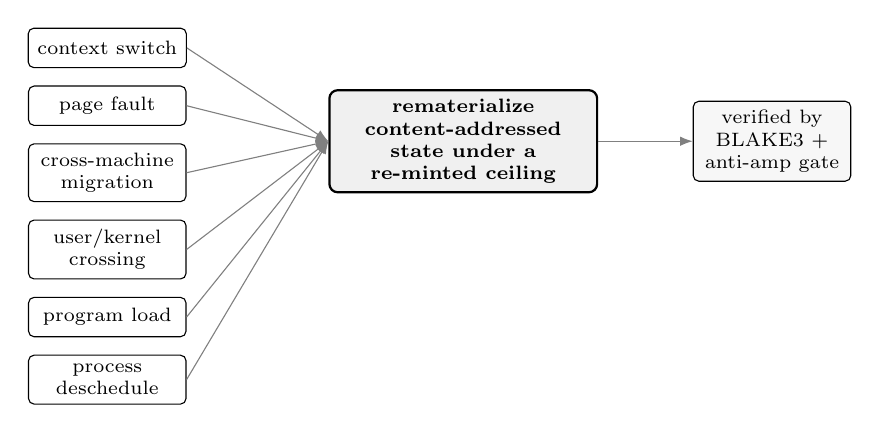
\begin{tikzpicture}[
  node distance=2.2mm,
  op/.style={draw, rounded corners=2pt, font=\scriptsize, align=center,
             minimum width=20mm, minimum height=5mm},
  core/.style={draw, thick, rounded corners=3pt, font=\scriptsize\bfseries,
               align=center, minimum width=34mm, minimum height=9mm, fill=black!6},
  ar/.style={-{Latex[length=1.6mm]}, gray}
]
\node[op] (cs) {context switch};
\node[op, below=of cs] (pf) {page fault};
\node[op, below=of pf] (mig) {cross-machine\\migration};
\node[op, below=of mig] (uk) {user/kernel\\crossing};
\node[op, below=of uk] (ld) {program load};
\node[op, below=of ld] (ds) {process\\deschedule};

\node[core, right=18mm of mig, yshift=4mm] (core)
  {rematerialize\\content-addressed\\state under a\\re-minted ceiling};

\foreach \n in {cs,pf,mig,uk,ld,ds} \draw[ar] (\n.east) -- (core.west);

\node[op, right=12mm of core, fill=black!3] (out)
  {verified by\\BLAKE3 +\\anti-amp gate};
\draw[ar] (core.east) -- (out.west);
\end{tikzpicture}}
\caption{The one-operation funnel. Six kernel operations on live execution
state are expressed as one operation, rematerialization of content-addressed
state under a re-minted capability ceiling, with integrity by BLAKE3 and
authority by the anti-amplification gate.}
\label{fig:funnel}
\end{figure}

\section{Architecture}

This section walks the system from the proven modules up through the kernel, and
ties each subsystem to the milestone in which it was observed. Milestone codes
(for example E2, R3, C3, M4) match the kernel self-test stages and the captured
serial transcript.

\subsection{Proven modules}

Five modules below the kernel hold the model and ship byte-identical to their
verified form.

\textbf{Capability model (cap/).} A capability is a record of a base, a length, a
permission set, and a validity tag. \emph{Strip} turns a live capability and a
reference to its referent into a plain descriptor carrying offset, length,
permissions, and the content hash of the referent, with no live authority tag.
\emph{Re-mint} takes a destination root, a descriptor, and the destination's copy
of the referent, and mints a fresh capability, checking in order that the
descriptor is well formed, that its bounds fit the source region, that its
permissions are a subset of the source, that write and execute are not both
requested, and that no forbidden permission is present. Any failure returns an
invalid capability.

\textbf{Content-addressed object store (store/).} The store maps a BLAKE3 hash to
bytes. Putting bytes returns their hash and stores one copy; putting identical
bytes again stores nothing new. The vendored BLAKE3 is validated against the
official known-answer vectors, and the kernel re-runs that known-answer check at
startup before it trusts any content-addressed result (milestone R0, digest of
the empty string matches \texttt{af1349b9..41f3262}).

\textbf{Single-level store and structural diff (sls/).} The single-level store
builds an object graph over the store. A leaf holds bytes; a node holds an ordered
list of child identities. Mutation produces a new object and a new epoch, and
unchanged sub-objects keep their identities. The structural diff takes two epoch
roots and returns the changed set, pruning any subtree whose hash is unchanged,
memoizing visited identity pairs, calling no hash function, and resolving only as
many objects as actually changed.

\textbf{WebAssembly safety gate (gate/).} The gate runs untrusted WebAssembly
under software fault isolation~\cite{wahbe1993sfi,haas2017wasm}. It validates a
WebAssembly subset, lowers it to a small typed intermediate representation, and
runs a linear-time checker that rejects any module that could escape its linear
memory or forge a capability. A static elision pass drops a runtime bounds check
only for an access it has proven in bounds, and the checker rejects the elided
opcodes in untrusted input so they cannot be injected.

\textbf{Software capability backend (carmix/).} The backend enforces the
capability model with no capability hardware. Its re-mint logic is the same
decision logic as cap/, ported to software records with integer comparisons and
no rounding. This backend is what the bootable kernel uses, and the binary
contains no capability instructions.

\subsection{Boot and in-kernel execution}

The kernel boots on x86-64 through the Limine boot protocol, which hands it long
mode, page tables, a memory map, and a linear framebuffer; everything above the
entry point is written for \carmix{}. The boot milestones B0 through B5 confirm
serial output, long mode (\texttt{CS=0x28}, \texttt{EFER.LMA=1}), a physical frame
allocator with read-back, a $1280\times800\times32$ framebuffer proven by pixel
read-back, and a PIT timer. The gate and the software backend, linked into the
kernel, run a WebAssembly task and draw its result (E1, result $=51$), and the
anti-amplification property holds in the kernel with one control accept and six
attack classes each rejected by its intended check (E2, $6/6$). The store and the
single-level store, linked in, checkpoint a counter and rematerialize it
bit-identically (R3), and demonstrate the diff-proportional structural diff (R4,
a one-leaf change reports one changed object, a self-diff reports zero, a
three-leaf change reports three).

\subsection{Desktop}

A software compositor draws a background and windows back to front with a
save-under cursor, driven by polled PS/2 keyboard and mouse. Windows support
focus raise on click, drag by the titlebar, and resize by a corner grip, each
proven by framebuffer pixel read-back. In the headless self-test run these events
are scripted and labelled as such; only the final shell stage takes live PS/2
input. The desktop draws \carmix{}'s own windows in software and does not run
third-party graphical applications.

\subsection{Two-machine migration and signed authorization}

Two emulator instances share memory through an ivshmem device used as a byte
channel. The migration is a destination-pull protocol: the source advertises its
epoch root, the destination walks the root top down and marks the hashes it
lacks, requests them, and verifies each block's BLAKE3 hash before installing it,
pruning any subtree it already holds. A block whose recomputed hash does not match
the requested hash is rejected fail-closed.

Hash verification proves integrity, not provenance. A signed authorization record
closes that gap. The record binds the migration to an epoch root, a computation
identifier, a destination identifier, an authority ceiling, a nonce, and an
expiry, and the source signs it with real Ed25519 (vendored
tweetnacl~\cite{bernstein2012nacl,bernstein2012ed25519}). Before it installs and
re-mints, the destination checks, each fail-closed with a distinct reason, that
the signature is valid under the expected source key, that the signed root equals
the root it pulled, that the destination and computation identifiers match, that
the nonce is unseen and unexpired, and finally that the re-mint is capped at the
authority ceiling through the anti-amplification gate. One legitimate migration is
accepted and seven adversaries are each rejected by their own reason (milestone
D2).

\subsection{Key lifecycle}

The destination holds a trust store of an authority public key, the current
source public key, a monotonic lifecycle epoch, and a permanent revoked set.
Authority-signed enrollment sets the first source key, rotation replaces it, and
revocation adds a key to the revoked set; a lifecycle record applies only if it
verifies under the authority key and its epoch strictly exceeds the stored epoch,
which rejects replay and downgrade. Each migration carries its signing key, which
must be the current source key and not revoked. Six lifecycle attacks are each
rejected by a distinct verdict (milestone KA). The destination's first authority
key is baked in; its bootstrap is out of scope and stated as such.

\subsection{The task substrate}

The kernel creates tasks and switches between them with a real assembly context
switch that saves and restores callee-saved registers and the stack pointer. A
cooperative yield calls it directly, and the timer interrupt calls it too, so a
task that never yields is still preempted (milestones P0 through P2). The
scheduling policy is isolated in one function, \texttt{pick\_next}, which is
round-robin and is a deliberate placeholder.

\subsection{The unified content-addressed task substrate}

On top of the substrate a task is made a content-addressed object. Its registers
and the used part of its stack hash into the proven store, the same state hashing
to the same handle and different state to a different handle (U0). Activate-by-hash
dematerializes the task to a hash and materializes it back, and the counter
survives the round trip (U1). Persistence falls out of this: a task dropped and
resumed from only its hash and the store resumes correctly, so the live and
durable forms are one object (U4). The cost is measured, not assumed. A raw
register switch is a flat cost near $1062$ cycles, while activate-by-hash costs
two to three orders of magnitude more at every dirty-set size, because hashing
dominates, with no dirty size at which it beats the register switch (U3). So the
fast switch stays the path for rapid preemption and content-addressing is used
only at coarse boundaries that already touch the store. The page-table root and
the capability slots are not yet part of the task state object.

\subsection{The residency manager}

Physical memory is managed as a content-addressed cache over the store. Fresh
allocation and mapping stay conventional; fault-in and sharing collapse into
rematerialization; free, eviction, and defragmentation partially collapse.
\texttt{materialize(hash)} fills a frame and verifies that its BLAKE3 equals the
requested hash, so integrity holds by construction (M2), a request for a resident
hash shares the existing frame and bumps its refcount, eviction writes a dirty
victim back before reuse with temporal victim selection (M3), and the hardware
page-table dirty bit is measured against the software chunk diff: both find the
same dirty set $\{1,4,6\}$ of eight pages and the hardware scan is roughly nine
times cheaper ($420{,}310$ against $3{,}956{,}943$ cycles, M4). Fixed chunks trade
external fragmentation for internal slack near $29$ percent on the measured mix,
and a frame-sized request stays serviceable (M5).

\subsection{The rematerializing fault handler}

Figure~\ref{fig:fault} shows the residency and fault path: a not-present access is
serviced as a verified materialize-by-hash, and a verification failure or a
protection fault is refused at the fault boundary.

\begin{figure}[t]
\centering
\resizebox{\columnwidth}{!}{%
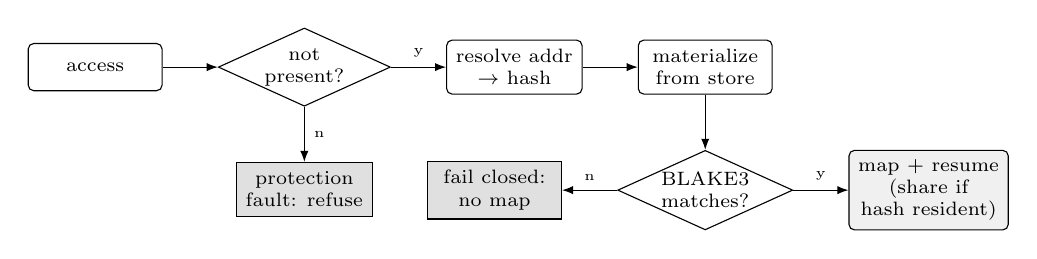
\begin{tikzpicture}[
  box/.style={draw, rounded corners=2pt, font=\scriptsize, align=center,
              minimum height=6mm, minimum width=17mm},
  dec/.style={draw, diamond, aspect=2.2, font=\scriptsize, align=center, inner sep=0.5pt},
  bad/.style={draw, font=\scriptsize, align=center, minimum height=6mm,
              minimum width=17mm, fill=black!12},
  ar/.style={-{Latex[length=1.4mm]}}
]
\node[box] (acc) {access};
\node[dec, right=7mm of acc] (np) {not\\present?};
\node[bad, below=7mm of np] (prot) {protection\\fault: refuse};
\node[box, right=7mm of np] (res) {resolve addr\\$\to$ hash};
\node[box, right=7mm of res] (mat) {materialize\\from store};
\node[dec, below=7mm of mat] (vf) {BLAKE3\\matches?};
\node[bad, left=7mm of vf] (fc) {fail closed:\\no map};
\node[box, right=7mm of vf, fill=black!6] (mp) {map + resume\\(share if\\hash resident)};

\draw[ar] (acc) -- (np);
\draw[ar] (np) -- node[above,font=\tiny]{y} (res);
\draw[ar] (np) -- node[right,font=\tiny]{n} (prot);
\draw[ar] (res) -- (mat);
\draw[ar] (mat) -- (vf);
\draw[ar] (vf) -- node[above,font=\tiny]{n} (fc);
\draw[ar] (vf) -- node[above,font=\tiny]{y} (mp);
\end{tikzpicture}}
\caption{The residency and fault path (F1, F2, F3). A miss is a verified
materialize-by-hash; a protection fault and a verification failure are each
refused at the fault boundary, and an already-resident hash is shared.}
\label{fig:fault}
\end{figure}

Demand paging is automatic. A not-present access traps through the page-fault
vector, the handler classifies the fault (a protection fault is not a miss),
resolves the faulting address to a content hash, materializes the object with
BLAKE3 verification, installs the mapping, and returns so the faulting instruction
re-executes (milestone F1, a live page fault). If the loaded bytes do not hash to
the expected hash, the handler installs no mapping and does not resume (F2). Two
addresses bound to one hash share one resident frame, so deduplication happens on
the fault path (F3). Two address-to-hash bindings were measured head to head and
the choice does not move fault-service latency, because the cost is dominated by
the materialize and the hash (F4, a null finding). The handler's own memory is
resident so servicing a miss does not itself fault; a fault during fault handling
fails closed rather than recovering, and making it recoverable needs a separate
interrupt stack and a per-fault service context, named as future work (F5).

\subsection{Authority-bounded user and kernel crossing}

The kernel runs a process in ring 3 on its own page tables, with a task-state
segment, a trap gate, and the user and supervisor bit on the page tables. A
ring-3 access to a kernel address faults and is classified as a protection
violation, not a miss (US0). Entering the kernel is not ambient privilege: a
privileged crossing re-mints the caller's bounded authority for the requested
service through the same anti-amplification gate that bounds a migration and a
fault, so a confused deputy that hands the kernel a wider claim is held to the
re-minted authority (US2). Six userspace amplification attempts, an unheld
capability, an over-ceiling request, a forged epoch, a confused deputy, a
write-execute violation, and a forbidden permission, are each refused by their own
distinct status code, the same codes the migration table uses, with a replay
refused and a legitimate crossing accepted (US3). A large syscall argument is
passed as a hash and rematerialized by hash with verification rather than copied,
which closes the copy-at-use class of time-of-check to time-of-use race, since a
mutated object is a different hash and fails verification; this relocates trust to
the address-to-hash binding and the store admission rather than eliminating it
(US4).

\subsection{The process loader}

A program is a content-addressed object and loading a process is materialization.
A freestanding ring-3 ELF64 is stored, the loader parses its program headers, and
for each loadable segment it materializes the bytes by hash with BLAKE3
verification into a fresh ring-3 address space, with the segment's permissions and
no segment both writable and executable (L1, W$\oplus$X held). The process runs
under a capability re-minted through the gate at load time, so its authority is
bounded at birth and an over-ceiling or unauthorized request is refused by the
same gate (L3, each refused by a distinct reason). Loading the same image twice
gives two processes whose read-only code resolves to one physical frame by hash
while their writable data and stacks are private (L4, code refcount $=3$). The
image is embedded in the kernel because there is no filesystem yet.

\subsection{Concurrency}

The scheduler runs more than one ring-3 process at once, each with its own
page-table root, instruction and stack pointers, and re-minted ceiling, and the
timer preempts and restores exactly (C0). Each process is bounded by its own
ceiling and neither can exercise the other's authority (C1). A descheduled process
is dematerialized to a hash and its frames released, so not running and not
resident become different states, and on reselection the state is rematerialized
with verification and the process resumes, its counter surviving (C2). The cost is
measured: resuming a resident process is a register and page-table-root restore
near $13{,}958$ cycles, and resuming a dematerialized process is a store fetch, a
verification, and a remap near $1{,}029{,}941$ cycles, about seventy times more on
this run, with the run-to-run variation expected under emulation (C3, see the
Evaluation). Today the register context and the private data page dematerialize
while the page-table root stays resident.

\subsection{The policy, fairness, and the heap}

A rematerialization-aware policy decides when to dematerialize. By default a
descheduled process is kept resident, since resuming it is far cheaper.
Dematerialization happens only under memory pressure when the process is predicted
to stay descheduled long enough to repay the rematerialize cost, with a break-even
duration computed live from the measured resume cost rather than a guessed
constant, and an anti-thrash backoff that keeps a just-rematerialized process
resident (milestones PP0 through PP4). A fairness control sits on top: a process
repeatedly paying the rematerialize cost accumulates a measured per-process
progress deficit, and a bounded keep-resident bias removes the penalty source so
its progress rate recovers without starving its resident peer (FA0 through FA2).
The control bounds future unfairness and recovers the rate; it does not refund the
penalty already paid and accounts for one peer rather than many, so it is a first
measured control on a lightly-researched dimension, not a proven-optimal
algorithm. A per-process heap grows through an authority-bounded extend-heap that
crosses the re-mint gate, backed demand-zero (PM0, PM1). An idle page can be
dematerialized to a hash and rematerialized on fault (PM2), two processes that
independently write the same bytes deduplicate to one frame by hash with
copy-on-write where copy-on-write structurally cannot, since there is no shared
ancestor (PM3), and a hot churning page is excluded from dematerialization because
re-hashing it on every attempt is the fine-granularity cost the residency
measurement showed (PM4).

\section{Trust Model and the Anti-Amplification Proof}

\subsection{Threat model}

The two-machine threat model covers tamper (a block corrupted in transit),
impersonation (a party that is not the legitimate source induces a
rematerialization), replay (an old signed migration presented again to force a
stale epoch), and scope escalation (state for a different computation,
destination, or higher ceiling). The signing key itself is a target, with unknown
key, rotation forgery, rotation replay or downgrade, use after revoke, and
revocation forgery. Hash verification closes tamper. The signed authorization
record closes impersonation and scope, and the key lifecycle closes the key
attacks, each fail-closed with a distinct reason as Section~3 and the Evaluation
report. Figure~\ref{fig:trust} shows the layered checks.

\begin{figure}[t]
\centering
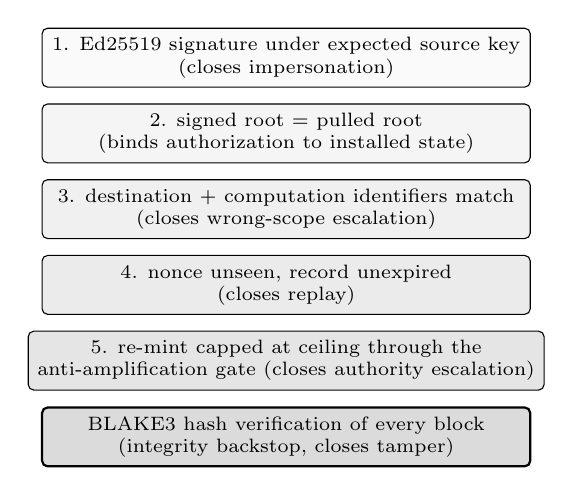
\begin{tikzpicture}[
  layer/.style={draw, rounded corners=2pt, font=\scriptsize, align=center,
                minimum width=62mm, minimum height=6mm},
  node distance=2mm
]
\node[layer, fill=black!2] (l1) {1. Ed25519 signature under expected source key\\(closes impersonation)};
\node[layer, below=of l1, fill=black!4] (l2) {2. signed root = pulled root\\(binds authorization to installed state)};
\node[layer, below=of l2, fill=black!6] (l3) {3. destination + computation identifiers match\\(closes wrong-scope escalation)};
\node[layer, below=of l3, fill=black!8] (l4) {4. nonce unseen, record unexpired\\(closes replay)};
\node[layer, below=of l4, fill=black!10] (l5) {5. re-mint capped at ceiling through the\\anti-amplification gate (closes authority escalation)};
\node[layer, below=of l5, fill=black!14, thick] (l6) {BLAKE3 hash verification of every block\\(integrity backstop, closes tamper)};
\end{tikzpicture}
\caption{The trust-model layers at the migration boundary. Each check is
fail-closed with a distinct reason, applied before any state is installed or any
capability is re-minted. The key-lifecycle current-key and not-revoked checks run
ahead of layer~1.}
\label{fig:trust}
\end{figure}

\subsection{The anti-amplification property}

The anti-amplification property is that a re-minted capability's base is no lower
and its limit no higher than the source region, and its permissions are a subset
of the source permissions. Figure~\ref{fig:gate} shows the gate. It is what makes
crossing, migrating, faulting, loading, and descheduling one authority model:
each goes through the same re-mint, and the gate is fail-closed, so over-authority
is rejected rather than clamped.

\begin{figure}[t]
\centering
\resizebox{\columnwidth}{!}{%
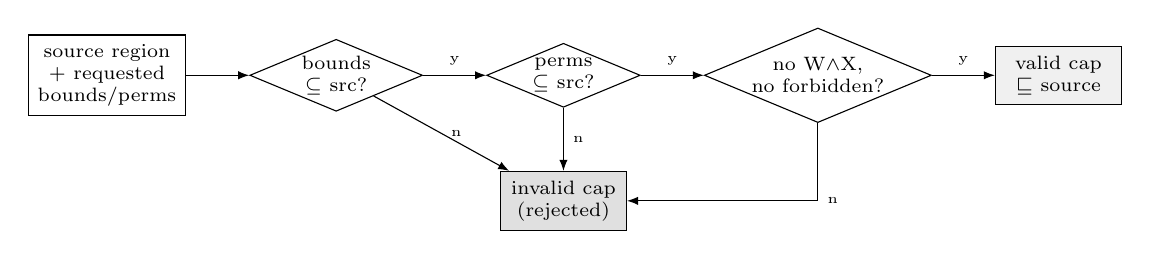
\begin{tikzpicture}[
  io/.style={draw, font=\scriptsize, align=center, minimum height=6mm, minimum width=20mm},
  chk/.style={draw, diamond, aspect=2.4, font=\scriptsize, align=center, inner sep=0.5pt},
  res/.style={draw, font=\scriptsize, align=center, minimum height=6mm, minimum width=16mm},
  ar/.style={-{Latex[length=1.4mm]}}
]
\node[io] (src) {source region\\+ requested\\bounds/perms};
\node[chk, right=8mm of src] (b) {bounds\\$\subseteq$ src?};
\node[chk, right=8mm of b] (p) {perms\\$\subseteq$ src?};
\node[chk, right=8mm of p] (wx) {no W$\land$X,\\no forbidden?};
\node[res, right=8mm of wx, fill=black!6] (ok) {valid cap\\$\sqsubseteq$ source};
\node[res, below=8mm of p, fill=black!12] (no) {invalid cap\\(rejected)};

\draw[ar] (src) -- (b);
\draw[ar] (b) -- node[above,font=\tiny]{y} (p);
\draw[ar] (p) -- node[above,font=\tiny]{y} (wx);
\draw[ar] (wx) -- node[above,font=\tiny]{y} (ok);
\draw[ar] (b) -- node[right,font=\tiny]{n} (no);
\draw[ar] (p) -- node[right,font=\tiny]{n} (no);
\draw[ar] (wx) |- node[right,font=\tiny]{n} (no);
\end{tikzpicture}}
\caption{The anti-amplification re-mint gate. Every authority crossing in
\carmix{}, migration, fault, user/kernel crossing, load, and deschedule, passes
through this one fail-closed gate.}
\label{fig:gate}
\end{figure}

\subsection{What the Coq development proves}

The proof in \texttt{proofs/Carmix.v} models a capability as a record of a base, a
limit, a finite permission set, and a validity flag, with a forbidden permission
subset. It defines an authority order in which one capability is below another
when its validity implies the other's, its range sits inside the other's, and its
permissions are a subset. It defines a re-mint function that clamps the requested
range to the source, intersects the requested permissions with the source, rejects
a request for write and execute together or for any forbidden permission, and sets
validity accordingly. Three results are machine-checked.

\begin{itemize}
\item \texttt{anti\_amplification}: for all sources and requests, if the re-minted
capability is valid then it is below the source in the authority order.
\item \texttt{valid\_dest\_no\_wx} and \texttt{valid\_dest\_no\_forbidden}: a valid
re-minted capability does not hold write and execute together and holds no
forbidden permission.
\item \texttt{acyclic\_graph}: the content-addressed object graph is acyclic.
\end{itemize}

The development is axiom-free except for one stated hypothesis. The acyclicity
result is scoped honestly: it does not derive acyclicity from hashing alone.
Objects are modeled as a finite inductive tree, a node carrying a payload and a
list of child objects, so a child is a strict subterm of its parent, a structural
size measure strictly decreases along the child relation, and acyclicity follows
from that well-founded order. The single hypothesis, that the identity function is
injective (collision resistance), is what connects the hash-graph back to that
finite tree. The size measure is a proven lemma, not an assumption. The
development contains no \texttt{Admitted}, no \texttt{admit}, and no
\texttt{Axiom}; \texttt{coqc} and \texttt{coqchk} both accept it, and an audit
reports the three authority results as closed under the global context and
\texttt{acyclic\_graph} as carrying only the collision-resistance hypothesis.

The proof is about the abstract capability algebra. It is not a proof that the C
implementation in \texttt{carmix/swcap.c} refines this model. The runtime
correspondence is demonstrated, not proven, by the kernel attack tables (E2, US3,
D2, KA), each of which runs the real software backend and observes each adversary
rejected by its intended check. A machine-checked refinement of the C code against
this model is future work.

\section{Evaluation}

All runtime numbers below were observed in the QEMU emulator and are quoted from
the captured serial transcript. Cycle counts are \texttt{rdtsc} differences taken
under TCG emulation, so they are noisy run to run; that variation is real and is
reported as such, and the point of each measurement is the order of magnitude and
the direction, not a precise constant.

\subsection{The cost crossover}

A raw register context switch is a flat cost near $1062$ cycles, independent of
dirty-set size (U3). Activate-by-hash, which serializes and hashes the task state,
is two to three orders of magnitude more at every swept dirty size, and there is
no dirty size at which it beats the register switch, because the BLAKE3 hash of
even one chunk already dwarfs the register swap. This is the load-bearing negative
result: a scheduling policy that content-addresses on every switch is not viable
on this hardware, so content-addressing is reserved for coarse, infrequent
boundaries that already touch the store. Table~\ref{tab:crossover} reports the
incremental-cost measurement (U2) that anchors it: re-storing only the dirty set
tracks the dirty set, with a one-chunk change far cheaper than a full re-store.

\begin{table}[t]
\centering
\caption{Incremental dematerialization tracks the dirty set (U2). A
$4096$-byte page in $16$ chunks; measured cycles are \texttt{rdtsc} under TCG.}
\label{tab:crossover}
\small
\begin{tabular}{lrrr}
\toprule
case & dirty chunks & bytes & cycles \\
\midrule
baseline (all dirty) & 16 & 4096 & 1{,}066{,}976 \\
small (1 chunk)      & 1  & 256  & 278{,}448 \\
large (all chunks)   & 16 & 4096 & 815{,}649 \\
\bottomrule
\end{tabular}
\end{table}

\subsection{Resume cost and the break-even}

The deschedule resume path was measured directly (C3). Resuming a resident
process, a register and page-table-root restore, cost $13{,}958$ cycles; resuming
a dematerialized process, a store fetch, a BLAKE3 verification, a writeback, and a
remap, cost $1{,}029{,}941$ cycles, a ratio near $73\times$ on this run. The
architecture narrative describes this path as about fifty times more expensive;
the spread between that figure and the $73\times$ measured here is the run-to-run
emulation noise the transcript notes explicitly. This single measured cost anchors
the policy. The break-even deschedule duration, the point past which freeing a
frame for the deschedule duration outweighs paying the extra resume cost, is
computed live from it at $493{,}223$ cycles (PP3). Table~\ref{tab:breakeven}
reports the net outcome across deschedule durations: shorter than the break-even
nets a loss, longer nets a gain. The anti-thrash backoff bounded a forced thrash
workload to a single dematerialization across seven rounds, keeping the process
resident on the other six (PP4).

\begin{table}[t]
\centering
\caption{Net outcome of dematerializing across deschedule duration, anchored in
the measured C3 resume cost (PP3). Net is freed-frame value over the deschedule
minus extra resume cost; break-even $D^\ast = 493{,}223$ cycles.}
\label{tab:breakeven}
\small
\begin{tabular}{rrrl}
\toprule
duration (cyc) & freed value & extra cost & verdict \\
\midrule
123{,}305   & 253{,}993   & 1{,}015{,}983 & loss \\
246{,}611   & 507{,}989   & 1{,}015{,}983 & loss \\
493{,}223   & 1{,}015{,}981 & 1{,}015{,}983 & loss \\
986{,}446   & 2{,}031{,}962 & 1{,}015{,}983 & gain \\
1{,}972{,}892 & 4{,}063{,}924 & 1{,}015{,}983 & gain \\
\bottomrule
\end{tabular}
\end{table}

\subsection{The dirty-bit comparison}

The unified-substrate crossover left open whether a cheap coarse filter could
front the content-addressing. The residency manager answers it (M4). A workload
wrote pages $\{1,4,6\}$ of eight. The hardware page-table dirty-bit scan and the
software \texttt{memcmp} chunk diff agree on the dirty set, and the hardware scan
cost $420{,}310$ cycles against the software diff's $3{,}956{,}943$, roughly nine
times cheaper. The hardware bit is the cheap coarse filter and content-addressing
is the fine mechanism, and they compose.

\subsection{Two-machine migration}

Table~\ref{tab:migration} reports the bytes on the wire between two emulator
instances. The cold sync transferred the full graph, $1093$ objects in $44{,}505$
bytes. Three warm hops after small changes transferred $1176$, $1176$, and $2219$
bytes; the third hop changed two leaves and fetched more than the first, which
changed one, so the warm transfer tracks each hop's own change set rather than a
constant. No block was rejected on these clean runs; a corrupted or forged block
is rejected fail-closed by the BLAKE3 hash check.

\begin{table}[t]
\centering
\caption{Two-machine diff-proportional migration, bytes on the wire, measured
between two emulator instances (milestones B2, B4).}
\label{tab:migration}
\small
\begin{tabular}{lrrr}
\toprule
sync & blocks & bytes received & store objects \\
\midrule
cold  & 1093 & 44{,}505 & 1093 \\
warm hop 1 & 4 & 1176 & 1097 \\
warm hop 2 & 4 & 1176 & 1101 \\
warm hop 3 & 7 & 2219 & 1108 \\
\bottomrule
\end{tabular}
\end{table}

\subsection{The adversarial tables}

The anti-amplification gate was run against attack classes at each boundary, and
each adversary was rejected by its own intended check, with a control accept.
Table~\ref{tab:adv} summarizes the runtime tables. The in-kernel anti-amp run
rejected $6/6$ (E2). The user and kernel boundary rejected six amplifications by
six distinct status codes plus a replay, with a legitimate crossing accepted
(US3). The migration trust boundary accepted one legitimate migration and rejected
seven adversaries each by a distinct reason (D2). The key lifecycle accepted the
legitimate enroll, rotate, and revoke flow and rejected six lifecycle attacks each
by a distinct verdict (KA). The status codes are shared across the boundaries,
which is the evidence that it is one gate.

\begin{table}[t]
\centering
\caption{Runtime adversarial tables. Each boundary runs the real software backend
and observes each adversary rejected by its intended check, with a control accept.}
\label{tab:adv}
\small
\begin{tabular}{llr}
\toprule
boundary & milestone & accept / reject \\
\midrule
in-kernel anti-amp & E2  & 1 / 6 \\
user/kernel crossing & US3 & 1 / 6 (+ replay) \\
two-machine migration & D2 & 1 / 7 \\
key lifecycle & KA & legit flow / 6 \\
\bottomrule
\end{tabular}
\end{table}

\subsection{Sharing and dedup}

Sharing a hash at admission re-materialized zero bytes and cost $116{,}891$
cycles, far less than a real fault at $2{,}456{,}493$ cycles per fault that moved
$4096$ bytes, so deduplicating on the way in beats a post-hoc merge (M2). On the
fault path two addresses bound to one hash shared one frame with a single store
fetch (F3). Two processes that independently wrote the same heap page, with no
shared ancestor, deduplicated to one physical frame by hash, and a later write
split a private copy under copy-on-write (PM3). A hot churning page is excluded
from dematerialization; over a burst of $64$ rewrites the exclusion avoided about
$26{,}689{,}536$ cycles of repeated hashing (PM4). The fairness measurement (FA0)
showed a process dematerialized every turn paying $12{,}191{,}796$ cycles of
rematerialize penalty over twelve equal turns that its resident peer did not pay,
and the keep-resident control stopped the deficit from climbing and recovered the
victim's progress rate (FA1, FA2).

\subsection{What the evaluation shows}

The measured advantage is repeated migration or deschedule of a large state with a
small change, where the transfer or the incremental store tracks the change. The
crossover and the resume cost show that content-addressing is not free and must be
confined to coarse boundaries, which is why the fast register switch stays the
common path. The dirty-bit result shows the cheap hardware filter composes with
the fine content mechanism. The adversarial tables show the one gate holds at every
boundary. None of this is a claim about raw compute speed, cold-start migration, or
operating-system completeness.

\section{Limitations}

\carmix{} is roughly forty to forty-five percent of the way to a general-purpose
operating system. The following are not built, and the list is the point of this
section.

\begin{itemize}
\item \textbf{No real hardware.} Everything runs in QEMU. The bootable image runs
the same path from a USB stick, but that has not been verified on a physical
machine, and there is no real network transport, only ivshmem shared memory
between two local instances.
\item \textbf{No filesystem or persistent storage.} The store is in RAM. There is
no storage driver, so a process image is embedded in the kernel and the trust and
nonce state do not survive a reboot.
\item \textbf{No full allocator.} A process can grow its heap through an
authority-bounded extend-heap backed demand-zero, and a userspace bump allocator
runs on the granted pages, but the bump allocator has no free, there are no huge
pages, and there is no production dedup-scan policy.
\item \textbf{No dynamic linking.} The loaded program is a static executable.
\item \textbf{Partial task-state dematerialization.} The content-addressed task
object today is the registers and the used stack only. The page-table root and the
capability slots stay resident and are not yet part of it.
\item \textbf{PM2 was serviced through the page-fault core directly.} The idle-page
rematerialization milestone calls the same C page-fault service routine the live
vector runs, rather than triggering a live fault on a freshly-unmapped low virtual
address, because a live touch there halts the boot on the single-stack handler.
The serial line says so on the wire, and the live page-fault entry is proven
separately by F1, US0, C0, and PM0.
\item \textbf{Recoverable nested faults are not supported.} A fault during fault
handling fails closed rather than recovering. Making it recoverable needs a
separate interrupt stack (IST/TSS) and a per-fault service context (F5).
\item \textbf{The fairness control rests on lighter research.} It bounds future
deficit growth and recovers the progress rate but does not refund the penalty
already paid, and it accounts for one peer rather than many. It is a first measured
control, not a proven-optimal fairness algorithm.
\item \textbf{The dedup side channel is named, not solved.} Content-addressed
deduplication across processes is a known timing and occupancy hazard, and \carmix{}
states it rather than mitigating it.
\item \textbf{The trust-root bootstrap is open.} The destination's first authority
public key is baked in. How a destination obtains and proves that first key,
through a certificate authority, identity proofing, or an out-of-band channel, is
the one irreducible bootstrap assumption and is not built. There is also no
trustworthy clock for the expiry check, only a tick counter, and one authority key
whose compromise is unrecoverable.
\item \textbf{Input is polled PS/2.} Real modern hardware needs a USB HID stack
over xHCI; the desktop is software-rendered and runs no third-party graphical
applications.
\item \textbf{The proof is the abstract algebra.} It is not a refinement of the C
code. The runtime correspondence is demonstrated by the attack tables, not proven.
\end{itemize}

\section{Related Work}

\textbf{Component and safe-language operating systems.} Theseus structures the
operating system as many small interchangeable cells with state ownership tracked
by the language, to make live evolution and fault recovery
tractable~\cite{boos2020theseus}. Twizzler builds an operating system around a
single global data-centric address space over persistent
memory~\cite{bittman2020twizzler}. Hubris is a small statically-defined
memory-protected embedded operating system with no dynamic task
creation~\cite{oxide2021hubris}. Unikraft composes a specialized unikernel from
modular library components~\cite{kuenzer2021unikraft}. \carmix{} differs by making
content-addressed rematerialization, not the module, the namespace, or the
language, the unit through which it expresses context switch, fault, migration,
crossing, load, and deschedule as one operation.

\textbf{Capability and microkernel systems.} seL4 is a microkernel with a complete
machine-checked functional-correctness proof and a capability access-control
model~\cite{klein2009sel4}. EROS and its ancestor KeyKOS are
capability-based systems with transparent orthogonal persistence by periodic
checkpoint~\cite{shapiro1999eros,hardy1985keykos}. Genode is a capability-based
component framework~\cite{feske2015genode}. \carmix{} shares the capability
discipline but adds the anti-amplification re-mint as a migration and crossing
primitive, ties it to a machine-checked authority property, and unifies it with
content-addressed transfer; its proof covers that authority algebra rather than
full kernel functional correctness.

\textbf{Migration and page deduplication.} MITOSIS migrates serverless function
state across machines efficiently~\cite{du2023mitosis}, and content-addressed or
hash-based virtual-machine and page migration has been built and measured. KSM
merges identical anonymous pages in Linux by content
scan~\cite{arcangeli2009ksm}. The nearest active project content-addresses program
binaries, naming a function by the hash of its code and sharing it across a
cluster. \carmix{} content-addresses live computation state, the running memory
graph, rather than code or post-hoc page scans, and re-mints the guarding
capabilities during the transfer, which the page-merge and binary-addressing lines
do not do.

\textbf{Content-addressed stores and hashing.} Git names objects by the SHA hash
of their content~\cite{git}, Nix builds a content-addressed package
store~\cite{dolstra2004nix}, and IPFS is a content-addressed distributed file
system~\cite{benet2014ipfs}. These address files, packages, and blocks at rest.
\carmix{} applies the same naming to live execution state and to physical-memory
residency. BLAKE3 is the hash function~\cite{blake3}, chosen for speed; the store
hashes only at commit and epoch boundaries, never in an execution loop.

\textbf{Replacement and working-set theory.} The residency manager and the
scheduling policy rest on the classical working-set model of program
locality~\cite{denning1968workingset}. \carmix{}'s contribution there is to anchor
the dematerialize decision in a measured rematerialize cost and a live break-even,
and to compose the hardware dirty bit with content-addressed dirty tracking, not a
new replacement algorithm.

The unoccupied axis is the synthesis. No prior system makes content-addressed
rematerialization under an authority-monotonic re-mint the single operation behind
context switch, fault, migration, crossing, load, and deschedule, with the
authority bound machine-checked.

\section{Conclusion and Future Work}

\carmix{} is a research operating system organized around one principle, that a
context switch, a page fault, a cross-machine migration, a user and kernel
crossing, a program load, and a process deschedule are one operation: the
rematerialization of content-addressed state under a re-minted anti-amplification
capability ceiling, over BLAKE3 hashes. The contribution is the principle and its
verified demonstration. The system boots, runs a capability-guarded WebAssembly
executor, rematerializes state on one machine and across two, enforces one
anti-amplification gate at every boundary with the adversarial tables to show it,
and machine-checks the core authority property in Coq under one stated
collision-resistance hypothesis. It is not a finished operating system, and the
Limitations section states what is missing.

Future work follows the open items. The proof should be extended to a
machine-checked refinement of the C backend against the abstract algebra, and a
verified BLAKE3 should replace the vendored one once a verified BLAKE3 is
confirmed to exist. The task-state object should grow to include the page-table
root and the capability slots, recoverable nested faults need an interrupt stack
and a per-fault service context, and the scheduling policy and the fairness control
need a learned predictor and a multi-peer treatment. The platform needs real
hardware bring-up, a USB HID stack, a persistent storage driver and filesystem, a
full allocator, dynamic linking, and a real network transport. The trust root
needs a bootstrap for the first authority key, persistent rollback-resistant trust
and nonce state, a trustworthy clock, and revocation at scale. Each of these is an
honest open item rather than a hidden one, and the credibility of the demonstrated
parts is meant to rest on that honesty.

\begin{thebibliography}{99}

\bibitem{ritchie1974unix}
D.~M. Ritchie and K.~Thompson.
The UNIX Time-Sharing System.
\emph{Communications of the ACM}, 17(7):365--375, 1974.

\bibitem{pike1995plan9}
R.~Pike, D.~Presotto, S.~Dorward, B.~Flandrena, K.~Thompson, H.~Trickey, and
P.~Winterbottom.
Plan 9 from Bell Labs.
\emph{Computing Systems}, 8(3):221--254, 1995.

\bibitem{wahbe1993sfi}
R.~Wahbe, S.~Lucco, T.~E. Anderson, and S.~L. Graham.
Efficient Software-Based Fault Isolation.
In \emph{Proceedings of the 14th ACM Symposium on Operating Systems Principles
(SOSP)}, pages 203--216, 1993.

\bibitem{haas2017wasm}
A.~Haas, A.~Rossberg, D.~L. Schuff, B.~L. Titzer, M.~Holman, D.~Gohman,
L.~Wagner, A.~Zakai, and J.~F. Bastien.
Bringing the Web up to Speed with WebAssembly.
In \emph{Proceedings of the 38th ACM SIGPLAN Conference on Programming Language
Design and Implementation (PLDI)}, pages 185--200, 2017.

\bibitem{bernstein2012nacl}
D.~J. Bernstein, T.~Lange, and P.~Schwabe.
The Security Impact of a New Cryptographic Library.
In \emph{Progress in Cryptology -- LATINCRYPT 2012}, LNCS 7533, pages 159--176,
2012.

\bibitem{bernstein2012ed25519}
D.~J. Bernstein, N.~Duif, T.~Lange, P.~Schwabe, and B.-Y. Yang.
High-Speed High-Security Signatures.
\emph{Journal of Cryptographic Engineering}, 2(2):77--89, 2012.

\bibitem{klein2009sel4}
G.~Klein, K.~Elphinstone, G.~Heiser, J.~Andronick, D.~Cock, P.~Derrin,
D.~Elkaduwe, K.~Engelhardt, R.~Kolanski, M.~Norrish, T.~Sewell, H.~Tuch, and
S.~Winwood.
seL4: Formal Verification of an OS Kernel.
In \emph{Proceedings of the 22nd ACM Symposium on Operating Systems Principles
(SOSP)}, pages 207--220, 2009.

\bibitem{shapiro1999eros}
J.~S. Shapiro, J.~M. Smith, and D.~J. Farber.
EROS: A Fast Capability System.
In \emph{Proceedings of the 17th ACM Symposium on Operating Systems Principles
(SOSP)}, pages 170--185, 1999.

\bibitem{hardy1985keykos}
N.~Hardy.
KeyKOS Architecture.
\emph{ACM SIGOPS Operating Systems Review}, 19(4):8--25, 1985.

\bibitem{feske2015genode}
N.~Feske.
\emph{Genode Operating System Framework Foundations}.
Genode Labs, 2015.

\bibitem{boos2020theseus}
K.~Boos, N.~Liyanage, R.~Ijaz, and L.~Zhong.
Theseus: An Experiment in Operating System Structure and State Management.
In \emph{Proceedings of the 14th USENIX Symposium on Operating Systems Design and
Implementation (OSDI)}, pages 1--19, 2020.

\bibitem{bittman2020twizzler}
D.~Bittman, P.~Alvaro, P.~Mehra, D.~D.~E. Long, and E.~L. Miller.
Twizzler: A Data-Centric OS for Non-Volatile Memory.
In \emph{Proceedings of the 2020 USENIX Annual Technical Conference (ATC)},
pages 65--80, 2020.

\bibitem{oxide2021hubris}
Oxide Computer Company.
Hubris: A Memory-Protected Microcontroller Operating System.
Technical documentation, 2021.

\bibitem{kuenzer2021unikraft}
S.~Kuenzer, V.-A. B\u{a}doiu, H.~Lefeuvre, S.~Santhanam, A.~Jung, G.~Gain,
C.~Soldani, C.~Lupu, S.~Teodorescu, C.~R\u{a}ducanu, C.~Banu, L.~Mathy,
R.~Deaconescu, C.~Raiciu, and F.~Huici.
Unikraft: Fast, Specialized Unikernels the Easy Way.
In \emph{Proceedings of the 16th European Conference on Computer Systems
(EuroSys)}, pages 376--394, 2021.

\bibitem{du2023mitosis}
D.~Du, Q.~Liu, X.~Jiang, Y.~Xia, B.~Zang, and H.~Chen.
Serverless Computing on Heterogeneous Computers with Fast Function Provisioning.
\emph{(MITOSIS / serverless function migration line of work)}, 2023.

\bibitem{arcangeli2009ksm}
A.~Arcangeli, I.~Eidus, and C.~Wright.
Increasing Memory Density by Using KSM.
In \emph{Proceedings of the Linux Symposium}, pages 19--28, 2009.

\bibitem{git}
S.~Chacon and B.~Straub.
\emph{Pro Git}.
Apress, 2nd edition, 2014.

\bibitem{dolstra2004nix}
E.~Dolstra, M.~de~Jonge, and E.~Visser.
Nix: A Safe and Policy-Free System for Software Deployment.
In \emph{Proceedings of the 18th USENIX Large Installation System Administration
Conference (LISA)}, pages 79--92, 2004.

\bibitem{benet2014ipfs}
J.~Benet.
IPFS -- Content Addressed, Versioned, P2P File System.
arXiv:1407.3561, 2014.

\bibitem{blake3}
J.~O'Connor, J.-P. Aumasson, S.~Neves, and Z.~Wilcox-O'Hearn.
\emph{BLAKE3: One Function, Fast Everywhere}.
Specification, 2020.

\bibitem{denning1968workingset}
P.~J. Denning.
The Working Set Model for Program Behavior.
\emph{Communications of the ACM}, 11(5):323--333, 1968.

\end{thebibliography}

\end{document}
